\documentclass[letterpaper,fleqn,leqno]{article}

\usepackage{amsmath}
\usepackage{amssymb}
\usepackage{enumerate}
\usepackage[letterpaper, margin=1in]{geometry}
\usepackage{tabularx}
%\usepackage{tikz}
\usepackage{pgfplots}
\usepackage{xcolor, colortbl}
\usepackage{mathrsfs}

\setlength{\extrarowheight}{3pt}

\begin{document}
	\newcommand{\problem}[2]{
		\noindent\textbf{Problem #1.} \\
		Exercise Set 7.#2
	}
	\newcommand{\chunk}[1]{
		\noindent\begin{minipage}[t]{\textwidth}
			#1
		\end{minipage}
	}
	\newcommand{\quess}[2]{
		\begin{enumerate}
			\item [#1.]
			#2
		\end{enumerate}
	}
	\newcommand{\ques}[2]{
		\begin{enumerate}
			\item [#1.] \quad
			#2
		\end{enumerate}
	}
	\newcommand{\union}[2] {
		\displaystyle \bigcup\limits_{#1}^{#2}
	}
	\newcommand{\inter}[2] {
		\displaystyle \bigcap\limits_{#1}^{#2}
	}
	\newcommand{\q}[1]{\stackrel{?}{#1}}

	\newcommand{\case}[2]{\cellcolor{yellow!25}\textbf{Case #1:} #2}

	\chunk{
		\problem{1}{1}
		\quess{28}{
			Student C tries to define a function $h:\mathbb{Q}\rightarrow\mathbb{Q}$ by the rule\\
			$h\left(\dfrac{m}{n}\right)=\dfrac{m^2}{n}$, for all integers $m$ and $n$ with $n\not=0$.\\
			Student D claims that $h$ is not well defined. Justify student D's claim.\\
			$\dfrac{1}{3}=\dfrac{2}{6}\Rightarrow h\left(\dfrac{1}{3}\right)=h\left(\dfrac{2}{6}\right)$\\
			$\left(h\left(\dfrac{1}{3}\right)=\dfrac{1}{3}\right)\not=\left(h\left(\dfrac{2}{6}\right)=\dfrac{4}{6}=\dfrac{2}{3}\right)$\\
			Contradiction, therefore $h$ is not well defined.\\
		}
	}
	\chunk{
		\problem{2}{1}
		\quess{35}{
			$F(A\cap B)\subseteq F(A)\cap F(B)$\\
			\textbf{Proof:}\\
			Suppose $y\in F(A\cap B)$.\\
			\textbf{Prove $y\in F(A)\cap F(B)$:}\\
			$y=F(x)$ for some $x\in A\cap B$.\\
			$x\in A$ by definition of intersection, therefore $y\in F(A)$.\\
			$x\in B$ by definition of intersection, therefore $y\in F(B)$.\\
			$y\in F(A)$ and $y\in F(B)$, therefore $y\in F(A) \cap F(B)$.\\
			Proof done. \\
		}
	}
	\chunk{
		\problem{3}{1}
		\quess{41}{
			For all subsets $C$ and $D$ of $Y$,\\
			$F^{-1}(C-D)=F^{-1}(C)-F^{-1}(D)$.\\
			\textbf{Proof:}
			\begin{itemize}
				\item []
				\textbf{Part 1: $F^{-1}(C-D)\subseteq F^{-1}(C)-F^{-1}(D)$}\\
				Suppose $x\in F^{-1}(C-D)$.\\
				\textbf{Prove $x\in F^{-1}(C)-F^{-1}(D)$:}\\
				$F(x)\in C-D$, therefore $F(x)\in C$ and $F(x)\notin D$.\\
				$x\in F^{-1}(C)$ and $x\not\in F^{-1}(D)$, therefore $x\in F^{-1}(C)-F^{-1}(D)$.\\
				Proof done.\\

				\item []
				\textbf{Part 2: $F^{-1}(C)-F^{-1}(D)\subseteq F^{-1}(C-D)$}\\
				Suppose $x\in F^{-1}(C)-F^{-1}(D)$.\\
				\textbf{Prove $x\in F^{-1}(C-D)$:}\\
				$x\in F^{-1}(C)$ and $x\not\in F^{-1}(D)$, therefore $F(x)\in C$ and $F(x)\notin D$.\\
				$F(x)\in C-D$, therefore $x\in F^{-1}(C-D)$.\\
				Proof done.\\
			\end{itemize}
			Both parts proven, therefore $F^{-1}(C-D)=F^{-1}(C)-F^{-1}(D)$.\\
		}
	}
	\chunk{
		\problem{4}{1}
		\quess{43}{
			Given a set $S$ and a subset $A$, the characteristic function of $A$, denoted $\chi_A$, is the function defined from $S$ to $\mathbb{Z}$ with the property that for all $u\in S$,\\
			$\chi_A(u)=\begin{cases}
				1 & \text{if $u\in A$}\\
				0 & \text{if $u\notin A$}\\
			\end{cases}$\\
			$A\subseteq S$, $B\subseteq S$, $u\in S$.
			\begin{enumerate}[(a)]
				\item $\chi_{A\cap B}(u)=\chi_A(u)\cdot\chi_B(u)$\\
				\begin{tabular}{|l|l|}
					\hline
					\case{1}{$u\notin A$ and $u\notin B$} & \case{2}{$u\notin A$ and $u\in B$}\\
					\hline
					$\chi_{A\cap B}(u)=0$ & $\chi_{A\cap B}(u)=0$\\
					$(\chi_A(u)=0)\cdot(\chi_B(u)=0)=0$ & $(\chi_A(u)=0)\cdot(\chi_B(u)=1)=0$\\
					$\chi_{A\cap B}(u)=\chi_A(u)\cdot\chi_B(u)$ & $\chi_{A\cap B}(u)=\chi_A(u)\cdot\chi_B(u)$\\
					Proof done. & Proof done.\\
					\hline
					\case{3}{$u\in A$ and $u\notin B$} & \case{4}{$u\in A$ and $u\in B$}\\
					\hline
					$\chi_{A\cap B}(u)=0$ & $\chi_{A\cap B}(u)=1$\\
					$(\chi_A(u)=1)\cdot(\chi_B(u)=0)=0$ & $(\chi_A(u)=1)\cdot(\chi_B(u)=1)=1$\\
					$\chi_{A\cap B}(u)=\chi_A(u)\cdot\chi_B(u)$ & $\chi_{A\cap B}(u)=\chi_A(u)\cdot\chi_B(u)$\\
					Proof done. & Proof done.\\
					\hline
				\end{tabular}\\
				$\chi_{A\cap B}(u)=\chi_A(u)\cdot\chi_B(u)$ is true in all cases.\\

				\item $\chi_{A\cup B}(u)=\chi_A(u)+\chi_B(u)-\chi_A(u)\cdot\chi_B(u)$\\
				\begin{tabular}{|l|l|}
					\hline
					\case{1}{$u\notin A$ and $u\notin B$} & \case{2}{$u\notin A$ and $u\in B$}\\
					\hline
					$\chi_{A\cup B}(u)=0$ & $\chi_{A\cup B}(u)=1$\\
					$\chi_A(u)=0, \chi_B(u)=0$ & $\chi_A(u)=0, \chi_B(u)=1$\\
					$\chi_A(u)+\chi_B(u)-\chi_A(u)\cdot\chi_B(u)=0$ & $\chi_A(u)+\chi_B(u)-\chi_A(u)\cdot\chi_B(u)=1$\\
					$\chi_{A\cap B}(u)=\chi_A(u)+\chi_B(u)-\chi_A(u)\cdot\chi_B(u)$ & $\chi_{A\cap B}(u)=\chi_A(u)+\chi_B(u)-\chi_A(u)\cdot\chi_B(u)$\\
					Proof done. & Proof done.\\
					\hline
					\case{3}{$u\in A$ and $u\notin B$} & \case{4}{$u\in A$ and $u\in B$}\\
					\hline
					$\chi_{A\cup B}(u)=0$ & $\chi_{A\cup B}(u)=1$\\
					$\chi_A(u)=1, \chi_B(u)=0$ & $\chi_A(u)=1, \chi_B(u)=1$\\
					$\chi_A(u)+\chi_B(u)-\chi_A(u)\cdot\chi_B(u)=1$ & $\chi_A(u)+\chi_B(u)-\chi_A(u)\cdot\chi_B(u)=1$\\
					$\chi_{A\cap B}(u)=\chi_A(u)+\chi_B(u)-\chi_A(u)\cdot\chi_B(u)$ & $\chi_{A\cap B}(u)=\chi_A(u)+\chi_B(u)-\chi_A(u)\cdot\chi_B(u)$\\
					Proof done. & Proof done.\\
					\hline
				\end{tabular}\\
				$\chi_{A\cap B}(u)=\chi_A(u)+\chi_B(u)-\chi_A(u)\cdot\chi_B(u)$ is true in all cases.\\
			\end{enumerate}
		}
	}
	\chunk{
		\problem{5}{2}
		\quess{23}{
			Define $H: \mathbb{R}^2\rightarrow\mathbb{R}^2$ as follows:\\
			$H(x,y)=(x+1,2-y)$ for all $(x,y)\in\mathbb{R}^2$.
			\begin{enumerate}[(a)]
				\item Is $H$ one-to-one?\\
				Suppose $(x_1,y_1)$ and $(x_2,y_2)\in\mathbb{R}^2$ and $H(x_1,y_1)=H(x_2,y_2)$.\\
				$H$ is one-to-one if $x_1=x_2$ and $y_1=y_2$.\\
				$(x_1+1,2-y_1)=(x_2+1,2-y_2)$\\
				$\begin{aligned}
					x_1+1 &= x_2+1\\
					x_1 &= x_2\\
				\end{aligned}$\quad
				$\begin{aligned}
					2-y_1 &= 2-y_2\\
					y_1 &= y_2\\
				\end{aligned}$\\
				$H$ is one-to-one.\\

				\item Is $H$ onto?\\
				Suppose $(a,b)\in\mathbb{R}^2$.\\
				$H$ is onto if there exists $(x,y)\in\mathbb{R}^2$ where $H(x,y)=(a,b)$.\\
				$(x+1,2-y)=(a,b)$\\
				$(x,y)=(a-1,2-b)\in\mathbb{R}^2$\\
				$\begin{aligned}
					H(x,y) &= H(a-1,2-b)\\
					&= ((a-1)+1, 2-(2-b))\\
					&= (a,b)\\
				\end{aligned}$\\
				$H$ is onto.\\
			\end{enumerate}
		}
	}
	\chunk{
		\problem{6}{2}
		\quess{29}{
			Prove that all real numbers $a$, $b$, and $x$ with $b$ and $x$ positive and $b\not=1$, $\log_b(x^a)=a\log_bx$.\\
			$\log_b(x^a)=a\log_bx$\\
			$\exp_b(\log_b(x^a))=\exp_b(a\log_bx)$\\\textbf{}
			$x^a=(\exp_b(\log_bx))^a$\\
			$x^a=x^a$\\
		}
	}
	\chunk{
		\problem{7}{3}
		\quess{11}{
			$H$ and $H^{-1}$ are both defined from $\mathbb{R}-\{1\}$ to $\mathbb{R}-\{1\}$ by the formula\\
			$H(x)=H^{-1}(x)=\dfrac{x+1}{x-1}$, for all $x\in\mathbb{R}-\{1\}$.\\
			$H(x)=H^{-1}(x)$ therefore $(H\circ H^{-1})(x)=(H^{-1}\circ H)(x)=(H\circ H)(x)$.\\
			$\begin{aligned}
				(H\circ H)(x) &= \dfrac{\frac{x+1}{x-1}+1}{\frac{x+1}{x-1}-1}\\
				&= \dfrac{\frac{x+1}{x-1}+\frac{x-1}{x-1}}{\frac{x+1}{x-1}-\frac{x-1}{x-1}}\\
				&= \dfrac{\frac{2x}{x-1}}{\frac{2}{x-1}}\\
				&= \dfrac{2x}{x-1}\cdot\dfrac{x-1}{2}\\
				&= x\\
			\end{aligned}$\\
			Both compositions produce the identity function.\\
		}
	}
	\chunk{
		\problem{8}{3}
		\quess{27}{
			Let $f: X\rightarrow Y$ and $g: Y\rightarrow Z$. Is the following property true or false? For all subsets $C$ in $Z$, $(g\circ f)^{-1}(C)=f^{-1}(g^{-1}(C))?$\\
			Let $h(x)=g(f(x))$.\\
			$h(x)=g(f(x))$\\
			$g^{-1}(h(x))=f(x)$\\
			$f^{-1}(g^{-1}(h(x)))=x$\\
			$h^{-1}(x)=(f^{-1}\circ g^{-1})(x)$ because $h^{-1}(h(x))=x$.\\
			$\begin{aligned}
				(g\circ f)^{-1}(C) &\q{=} f^{-1}(g^{-1}(C))\\
				(g(f(x)))^{-1}(C) &\q{=} (f^{-1}\circ g^{-1})(C))\\
				h^{-1}(C) &= h^{-1}(C)\\
			\end{aligned}$\\
			Property is true.\\
		}
	}
	\chunk{
		\problem{9}{4}
		\quess{12}{
			Let $a$ and $b$ be real numbers with $a<b$, and suppose that $W=\{x\in\mathbb{R} \mid a<x<b\}$. Prove that $S$ and $W$ have the same cardinality.\\
			$S=(0,1)$ and $W=(a,b)$.\\
			Let $F(x)=\dfrac{x-a}{b-a}$. \\
			When $x\in W$, $a<x<b$.\\
			$F(a)<F(x)<F(b) \Rightarrow 0<F(x)<1$.\\
			$F(W)=S$, therefore $F: W\rightarrow S$.\\
			\begin{tabular}{|l|l|}
				\hline
				\cellcolor{green!25}\textbf{Injective} & \cellcolor{green!25}\textbf{Surjective}\\
				\hline
				\begin{tabular}[t]{l}
					Suppose $x_1$ and $x_2\in\mathbb{R}$ and $F(x_1)=F(x_2)$.\\
					$F$ is one-to-one if $x_1=x_2$.\\
					$\begin{aligned}
						F(x_1) &= F(x_2)\\
						\dfrac{x_1-a}{b-a} &= \dfrac{x_2-a}{b-a}\\
						x_1-a &= x_2-a\\
						x_1 &= x_2\\
					\end{aligned}$\\
					F is one-to-one.\\
				\end{tabular} &
				\begin{tabular}[t]{l}
					Suppose $y\in S$.\\
					$F$ is onto if there exists $x\in W$ where $F(x)=y$.\\
					$\begin{aligned}
						\dfrac{x-a}{b-a} &= y\\
						x &= y(b-a)+a\\
					\end{aligned}$\\
					$0<y<1$\\
					$0<y(b-a)<b-a$\\
					$a<y(b-a)+a<b$\\
					$a<x<b$\\
					$x\in W$\\
					$\begin{aligned}
						F(y(b-a)+a) &= \dfrac{(y(b-a)+a)-a}{b-a}\\
						&= \dfrac{y(b-a)}{b-a}\\
						&= y\\
					\end{aligned}$\\
					F is onto.\\
				\end{tabular}\\
				\hline
			\end{tabular}\\
			$F: W\rightarrow S$ and is one-to-one and onto, therefore $W$ and $S$ have the same cardinality.\\
		}
	}
	\chunk{
		\problem{10}{4}
		\quess{20}{
			Give two examples of functions from $\mathbb{Z}$ to $\mathbb{Z}$ that are one-to-one but not onto.
			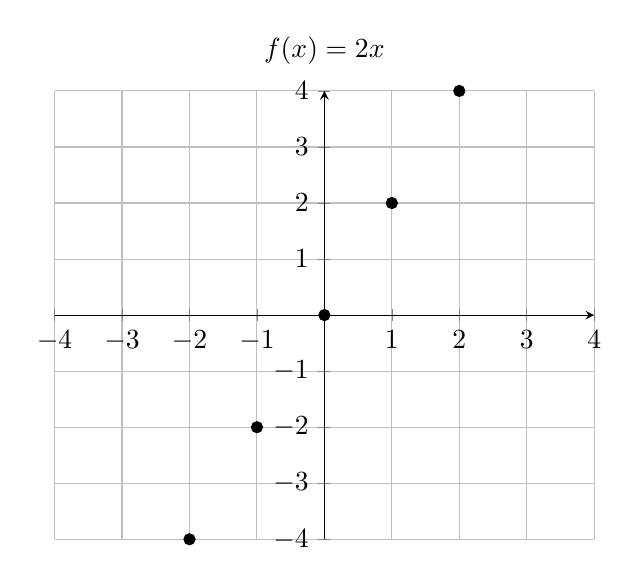
\begin{tikzpicture}
				\begin{axis}[
					title={$f(x)=2x$},
					xmin=-4, xmax=4,
					ymin=-4, ymax=4,
					xtick={-4,...,4},
					ytick={-4,...,4},
					axis lines=middle,
					grid=major
				]
				\foreach \i in {-4,...,4}{
					\addplot [mark=*] coordinates {(\i, \i*2)};
				}
				\end{axis}
			\end{tikzpicture}
			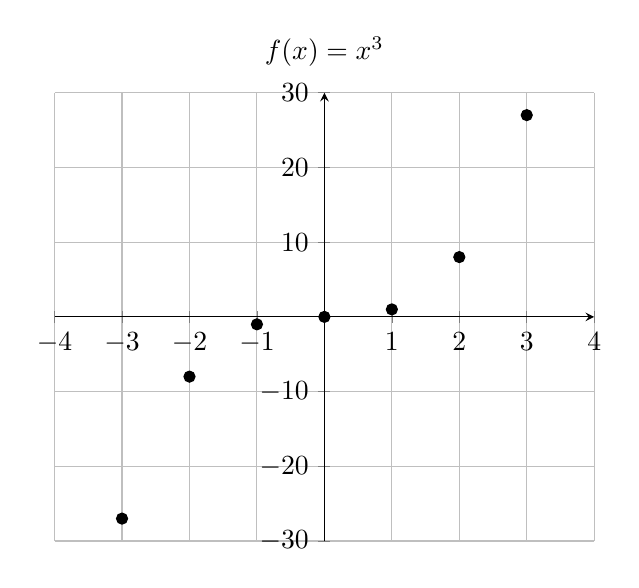
\begin{tikzpicture}
				\begin{axis}[
					title={$f(x)=x^3$},
					xmin=-4, xmax=4,
					ymin=-30, ymax=30,
					xtick={-4,...,4},
					ytick={-30,-20,...,30},
					axis lines=middle,
					grid=major
					]
					\foreach \i in {-4,...,4}{
						\addplot [mark=*] coordinates {(\i, \i^3)};
					}
				\end{axis}
			\end{tikzpicture}
		}
		\quess{21}{
			Give two examples of functions from $\mathbb{Z}$ to $\mathbb{Z}$ that are onto but not one-to-one.
			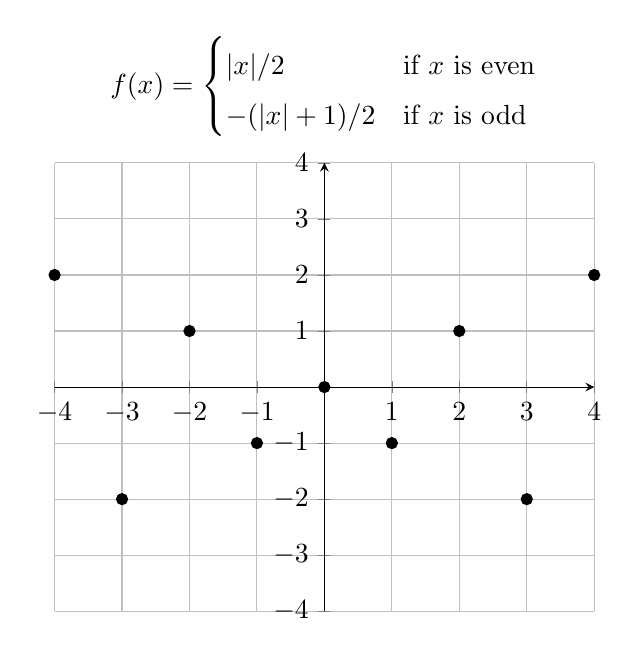
\begin{tikzpicture}
				\begin{axis}[
					title={$f(x)=\begin{cases}
							|x|/2 & \text{if $x$ is even}\\
							-(|x|+1)/2 & \text{if $x$ is odd}\\
						\end{cases}$},
					xmin=-4, xmax=4,
					ymin=-4, ymax=4,
					xtick={-4,...,4},
					ytick={-4,...,4},
					axis lines=middle,
					grid=major
					]
					\foreach \i in {-4,-2,...,4}{
						\addplot [mark=*] coordinates {(\i, {abs(\i)/2})};
					}
					\foreach \i in {-3,-1,...,3}{
						\addplot [mark=*] coordinates {(\i, {-(abs(\i)+1)/2})};
					}
				\end{axis}
			\end{tikzpicture}
			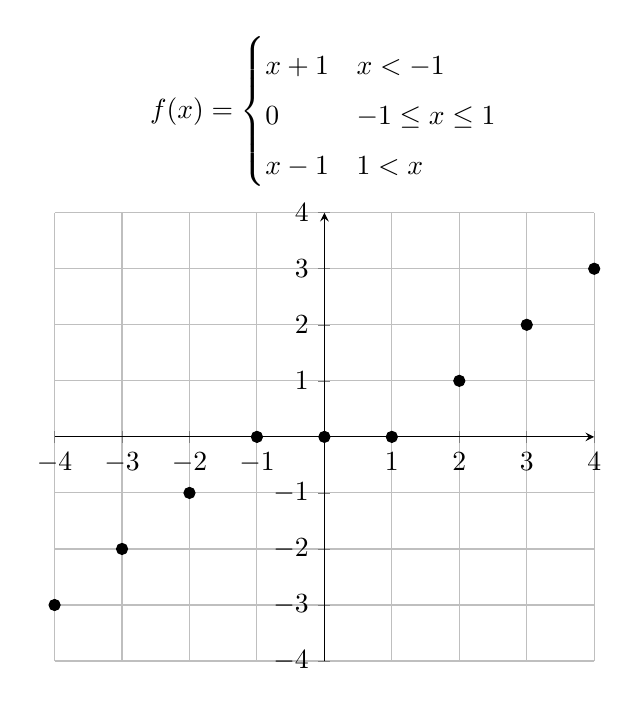
\begin{tikzpicture}
				\begin{axis}[
					title={$f(x)=\begin{cases}
							x+1 & x<-1\\
							0 & -1\leq x\leq1\\
							x-1 & 1<x\\
						\end{cases}$},
					xmin=-4, xmax=4,
					ymin=-4, ymax=4,
					xtick={-4,...,4},
					ytick={-4,...,4},
					axis lines=middle,
					grid=major
					]
					\foreach \i in {-4,...,-2}{
						\addplot [mark=*] coordinates {(\i, \i+1)};
					}
					\foreach \i in {-1,0,1}{
						\addplot [mark=*] coordinates {(\i, 0)};
					}
					\foreach \i in {2,...,4}{
						\addplot [mark=*] coordinates {(\i, \i-1)};
					}
				\end{axis}
			\end{tikzpicture}
		}
	}
\end{document}